\documentclass[a4paper, 12pt]{article}
\usepackage{graphicx}
\usepackage{hyperref}
\usepackage{amsmath, amsthm}

\usepackage[T1]{fontenc}
\usepackage[full]{textcomp}

%\usepackage{arev}
%\usepackage{fourier}
%\usepackage{fouriernc}
%\usepackage[utopia]{mathdesign}
%\usepackage[garamond]{mathdesign}
\usepackage[charter]{mathdesign}
%\usepackage{kpfonts}

%\usepackage{times}           % Times + Helvetica + Courier + Symbol 
%\usepackage{mathptmx}        % Times + Helvetica + Courier + Times Math
%\usepackage{mathpazo}        % Palatino + Helvetica + Courier + Palatino 
%\usepackage{newcent}         % New Century Schoolbook + Avant Garde + Courier
%\usepackage{bookman}         % Bookman + Avant Garde + Courier

%\DeclareGraphicsExtensions{.eps , .pdf}

\usepackage{fullpage}
%\setlength{\topmargin}{0 cm}
%\setlength{\headheight}{-2.5 cm}
%\setlength{\headsep}{0 cm}
%\advance\textheight by 4.0 cm
%\advance\textwidth by 2.0 cm
%\advance\oddsidemargin by -1.0 cm
%\advance\evensidemargin by -1.0 cm

\newcommand{\Mod}[1]{\ (#1)}
\DeclareMathOperator{\cand}{cand}

\setlength{\parindent}{0cm}
%\sloppy
%\pagestyle{plain}

\newcommand\T{\rule{0pt}{2.6ex}}
\newcommand\B{\rule[-1.4ex]{0pt}{0pt}} 

\usepackage{titlesec}
\titleformat*{\section}{\large\bfseries}

\theoremstyle{plain}
\newtheorem*{theorem}{Theorem}
\newtheorem*{lemma}{Lemma}
\newtheorem*{conjecture}{Conjecture}

\theoremstyle{definition}
\newtheorem*{examples}{Examples}
\newtheorem*{definition}{Definition}

\title{Quad Sieve for twin and Sophie Germain primes}
\author{Yves Gallot}
%\date{}

\begin{document}
\maketitle
%\thispagestyle{empty}

If we search for twin and Sophie Germain prime numbers, we first test the primality of $k\,2^n - 1$.
If it is prime, then we check the primality of $k\,2^n + 1$, $k\,2^{n-1} - 1$ and $k\,2^{n+1} - 1$.
A quad sieve ensures that the four forms don't have any small prime divisor.

\medskip

Based on Bateman and Horn conjecture, the expected numbers of remaining candidates,
primes of the form $k\,2^n - 1$, twin primes and of Sophie Germain primes in a fixed
sieved range are calculated in this note. 

\begin{conjecture}[Bateman and Horn]$ $\\
Let $f_1, f_2, \cdots, f_m$ be a set of $m$ distinct irreducible polynomials
with integral coefficients and a positive leading coefficient.
Let $f$ be their product and suppose that $f$does not vanish identically modulo any prime. 
Let $w(p)$ be the number of solutions to the congruence $f(x) \equiv 0 \pmod p$.\\
An integer $n$ is prime-generating if every polynomial $f_i(n)$ produces a prime number.\\
$\pi_f$ is the number of prime-generating integers for $n_1 \leq n \leq n_2$.
If $n_2 - n_1 \to \infty$ then
\begin{equation*}
\begin{split}
\pi_f \quad
 &\sim \quad C_f \sum_{n = n_1}^{n_2} \frac{1}{\log f_1(n) \cdot \log f_2(n) \cdots \log f_m(n)} \\
 &\sim \quad \frac{C_f}{D_f} \int_{n_1}^{n_2} \frac{dt}{\left(\log t\right)^m}\\
 &\sim \quad \frac{C_f}{D_f} \left( \frac{n_2}{\left(\log n_2\right)^m}
           - \frac{n_1}{\left(\log n_1\right)^m}\right),
\end{split}
\end{equation*}
where $D_f$ is the product of the degrees of the polynomials $f_1, f_2, \cdots, f_m$ and
\[C_f = \prod_{p\text{ prime}} \frac{1 - w(p)/p}{\left(1 - 1/p\right)^m}.\]
\end{conjecture}

\medskip

$C_f$ is a sieving constant. Let $S$ be a set containing $n$ $m$-tuples of random integers.
$S$ is sieved for $p \leq p_{max}$: an element is removed from the set if at least one
integer of the $m$-tuple is divisible by $p$. The expected number of remaining elements
is $\prod_{p\leq p_{max}}\left(1 - 1/p\right)^m\,n$. If the $m$-tuples of the set are
generated with the polynomials $f_i$ then the expected number of remaining elements
is $\cand_{p_{max}}(n) = \prod_{p\leq p_{max}}\left(1 - w(p)/p\right)\,n$.

\medskip

$k\,2^n - 1$ is odd and $C_{k\,2^n - 1} = 2$.

\medskip

For twin primes, we have $f_1(x) = 2\,x - 1$ and $f_2(x) = 2\,x + 1$. $w(2) = 0$ and
$w(p) = 2$ for $p > 2$. $C_{(k\,2^n - 1,\, k\,2^n + 1)} = 4\,C_2$, where $C_2$ is the
twin prime constant.\\
$C_{(k\,2^n - 1,\, k\,2^n + 1)} \approx 2.6406473$.

\medskip

$f_1(x) = 2\,x - 1$ and $f_2(x) = 4\,x - 1$ for Sophie Germain primes. We still have $w(2) = 0$ and
$w(p) = 2$ for $p > 2$ then  $C_{(k\,2^n - 1,\, k\,2^{n+1} - 1)} = C_{(k\,2^n - 1,\, k\,2^n + 1)}$.

\medskip

The functions of the quadruplet are $f_1(x) = 2\,x - 1$, $f_2(x) = 4\,x - 1$, $f_3(x) = 8\,x - 1$
and $f_4(x) = 4\,x + 1$. $w(2) = 0$, $w(3) = 2$ and $w(p) = 4$ for $p > 3$.\\
$C_{(k\,2^{n-1} - 1,\, k\,2^n - 1,\, k\,2^{n+1} - 1,\, k\,2^n + 1)} \approx 8.3023617$.

\medskip

In the following table, the formula with the summation is applied.
\begin{center}
Number of prime patterns: $k$ is odd, $1 \leq k \leq 10^8$
\smallskip

\begin{tabular}{llrr}
& Form & Actual & Expected.\\
\hline \T
single & $8\,k - 1$ & 5143331 & 5143482.8\\
twin & $8\,k - 1, 8\,k + 1$ & 350779 & 350497.4\\
Sophie Germain I & $4\,k - 1, 8\,k - 1$ & 363795 & 363558.9 \\
Sophie Germain II & $8\,k - 1, 16\,k - 1$ & 338858 & 338346.4\\
quadruplet & $4\,k - 1, 8\,k - 1, 8\,k + 1, 16\, k - 1$ & 3042 & 2978.2
\end{tabular}
\end{center}

\medskip

Mertens' third theorem is $\lim_{n \to \infty} \log n\, \prod_{p \leq n} \left(1 - 1/p\right)
= e^{-\gamma},$ where $\gamma \approx 0.57721566$ is the Euler's constant.

We have $\cand_{p_{max}}(n) = \prod_{p\leq p_{max}}\left(1 - w(p)/p\right)\,n
\approx C_f \prod_{p\leq p_{max}}\left(1 - 1/p\right)^m\,n$, hence
\[\cand_{p_{max}}(n) \approx C_f\, \left(\frac{e^{-\gamma}}{\log p_{max}}\right)^m\, n.\]

For quad sieve, we have
\[\cand_{p_{max}}(n) \approx \frac{0.82504063\, n}{\left(\log p_{max}\right)^4}.\]

\medskip
 
If $N$ has no prime factor $p \leq p_{max}$ then the likelihood that $N$ is prime is
\[\mathcal{P}(N) = \prod_{p \leq p_{max}} \left(1 - 1/p\right)^{-1} \frac{1}{\log N}
 \approx \frac{\log p_{max}}{e^{-\gamma} \log N}.\]

Let $S$ be a set of pairs $(k,\, n)$. A quad sieve is applied to this set. The expected
number of primes is
\[\pi_{k\,2^n - 1} \approx \frac{1.4694571}{\left(\log p_{max}\right)^3}
 \sum_S \frac{1}{\log(k\,2^n - 1)} .\]
If $n$ is fixed and $k$ is odd, $k_1 \leq k \leq k_2$ and $1 \ll k\,2^n$, we have:
\[\pi_s \approx \frac{0.73472856}{\left(\log p_{max}\right)^3}
 \int_{k_1}^{k_2} \frac{dt}{\log(t\,2^n)}.\]

Applying $\mathcal{P}(N)$ twice for twin primes, we obtain
\[\pi_t \approx \frac{1.30860477}{\left(\log p_{max}\right)^2}
 \int_{k_1}^{k_2} \frac{dt}{\log(t\,2^n)^2},\]
 and $\pi_{SG} \approx 2\,\pi_t$.

\begin{center}
Quad sieve prime occurrences:\\
\bigskip

$p_{max} = 10^4$, $n = 100$, $k$ is odd, $1 \leq k \leq 10^9$
\smallskip

\begin{tabular}{lrr}
 & Actual & Expected.\\
\hline \T
candidates & 57069 & 57324.8\\
primes & 10461 & 10562.8\\
twin & 1950 & 1946.6\\
Sophie Germain & 3825 & 3893.2
\end{tabular}
\bigskip

$p_{max} = 10^5$, $n = 100$, $k$ is odd, $1 \leq k \leq 10^9$
\smallskip

\begin{tabular}{lrr}
 & Actual & Expected.\\
\hline \T
candidates & 23660 & 23480.2\\
primes & 5419 & 5408.2\\
twin & 1280 & 1245.8\\
Sophie Germain & 2481 & 2491.6
\end{tabular}
\bigskip

$p_{max} = 10^5$, $n = 1000$, $k$ is odd, $1 \leq k \leq 10^{10}$
\smallskip

\begin{tabular}{lrr}
 & Actual & Expected.\\
\hline \T
candidates & 234241 & 234802.4\\
primes & 6784 & 6732.2\\
twin & 175 & 193.0\\
Sophie Germain &392 & 386.1
\end{tabular}
\bigskip

\end{center}

If $n = 3321925$ then $k\,2^n - 1$ has more than one million digits.
For $1 \leq k \leq 2^{52}$ the expected values are
\begin{center}
\begin{tabular}{ccccc}
$p_{max}$ & candidates & primes & twin & SG \B\\
\hline \T
$10^{12}$ & 3,187,000,000 & 68,120 & 1.46 & 2.91 \B \\
$10^{13}$ & 2,314,000,000 & 53,578 & 1.24 & 2.48 \B \\
$10^{14}$ & 1,720,000,000 & 42,898 & 1.07 & 2.14 \B \\
$10^{15}$ & 1,306,000,000 & 34,877 & 0.93 & 1.86
\end{tabular}
\bigskip
\end{center}

In practice, we can set $3321925 \leq n \leq 3321925 + 63$ and $1 \leq k \leq 2^{46}$.
The subset $1 \leq k \leq 2^{32}$ was sieved for $p_{max} < 10^{12}$. 194535 candidates
were expected and 195115 remain. 

\medskip

If the range is sieved to $10^{15}$ on GPU and that the number of mega-primes found
each year is still growing at the same rate then a mega twin prime could be discovered
within the next ten years.

\begin{center}
Number of known mega-primes per year
\par\nobreak
\smallskip
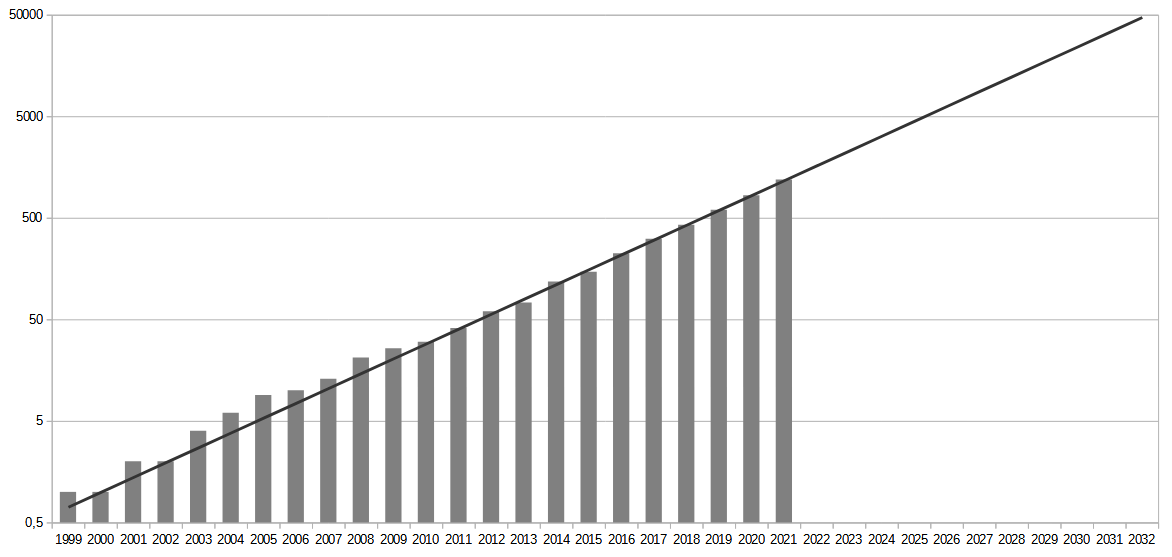
\includegraphics[scale=1.6]{mega_year.png}
\end{center}

\end{document}
